%----------------------------------------------------------------------------------------
%	SECTION 3
%----------------------------------------------------------------------------------------

\section{Future Career Aspirations} \label{sec:future}

%\hl{Future aspirations.}
%I think I would like to build my career in Sweden because it is a safe and profitable (?) place to work and live with many benefits, e.g. parental leave, and I would be close to my family.
%I would really like to work towards improving the sustainability of buildings.
%Sweden is pretty well known for their environmentally conscious efforts and their sustainability, e.g. with their recycling, their district heating systems, their high building standards with regards to U-values etc.
%I think I could learn a lot about increasing sustainability in the built environment by working for an environmentally responsible construction or consulting company in Sweden.
%Perhaps after that I will stay/ remain in Sweden or share my knowledge somewhere else in the world where it is more needed.
%This is why I looked for a summer placement in Sweden this year, so I could ``get my foot in the door", make contacts and find opportunities for work once I graduate next year.

I think a job feels fulfilling if it meets an external need, as opposed to just serving oneself or doing something pleasurable.
I have therefore paid attention to needs that Architectural Engineers can help fulfil.
%Paying attention to the needs of the built environment
These include the needs to mitigate and adapt to climate change,
and to improve collaborative workflows in the construction industry to increase productivity.
I investigated the latter for my dissertation and it felt fulfilling.


\begin{wrapfigure}{r}{0.4\textwidth}
	\centering
	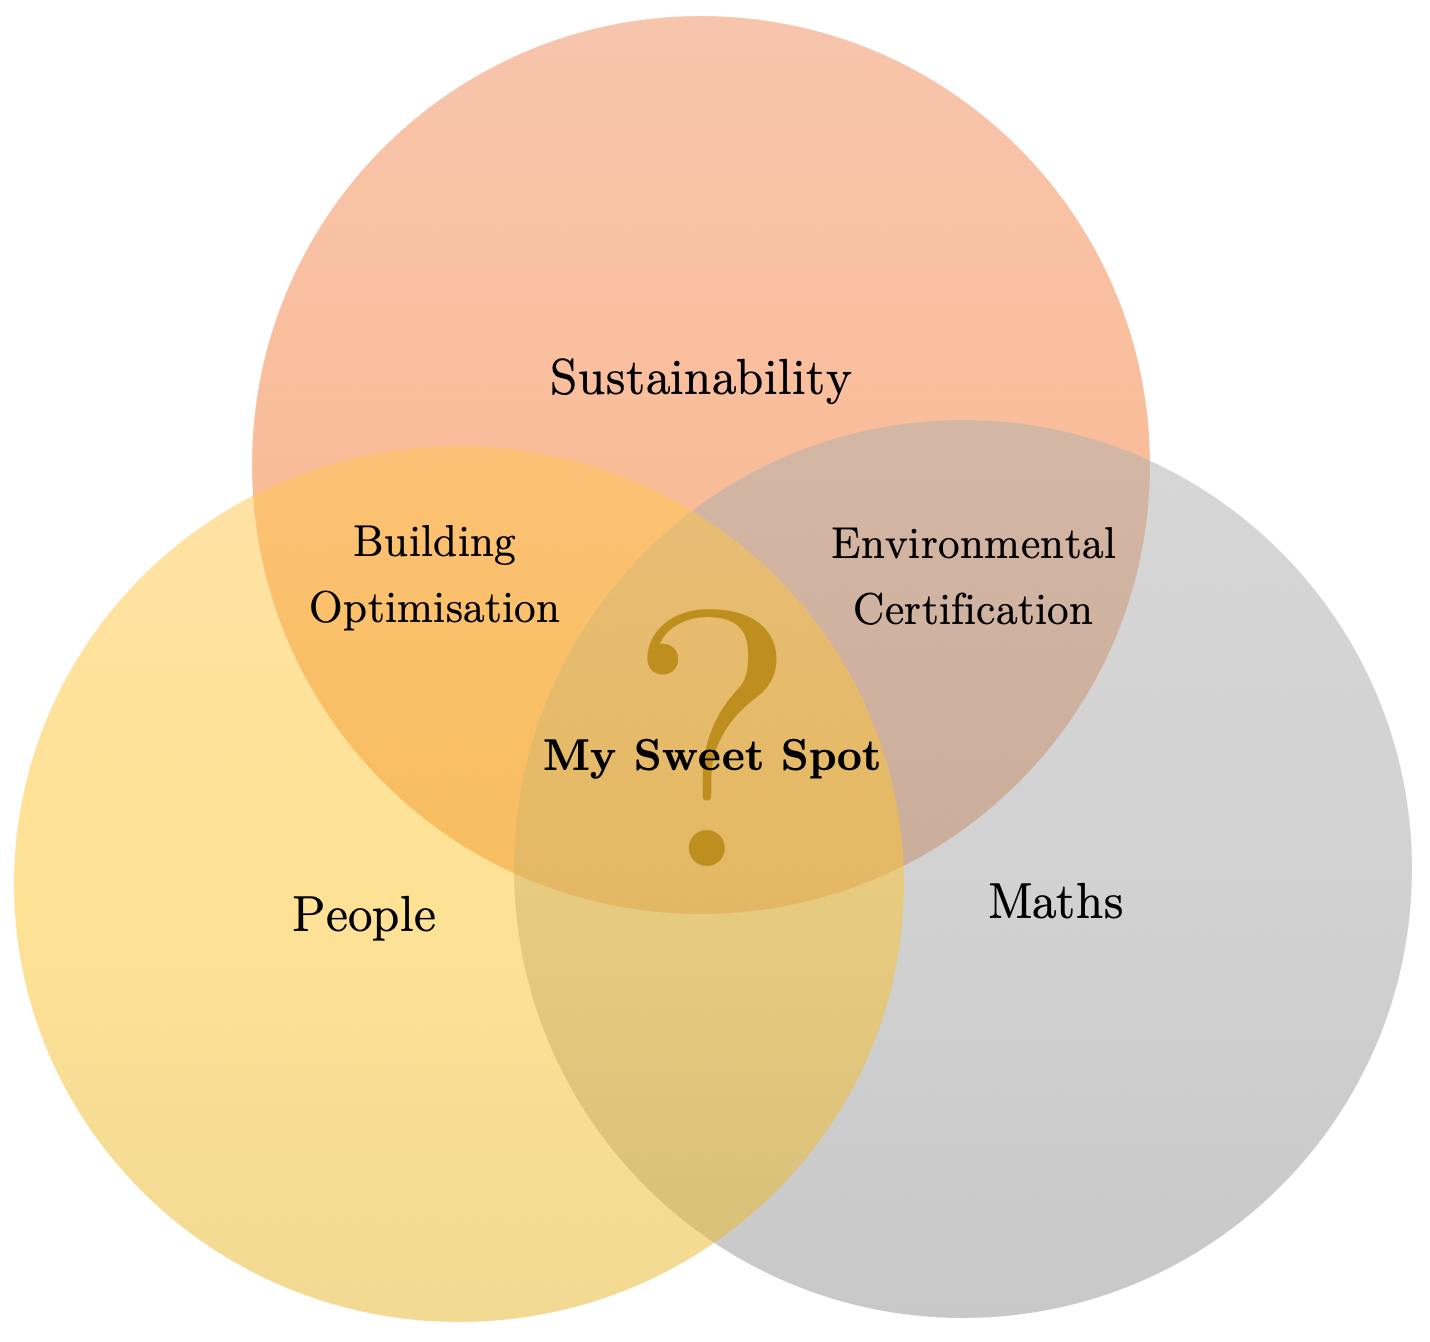
\includegraphics[width=0.4\textwidth]{figures/sweetspot2.png}
	\rule{0.4\textwidth}{0.5pt} % use line???
	\caption{My ideal career `sweet spot'.}
	\label{fig:sweetspot}
\end{wrapfigure}


Analysing the reasons that I particularly enjoyed certain courses has helped me narrow down the characteristics of my ideal career.
Courses such as \HBETitle \space and \IDTitle \space confirmed \textbf{my admiration for the built environment} and my selection of the AE programme.
Learning how building design and innovation can meet needs like mitigating and adapting to climate change in courses such as \IETitle, \EnBldgsTitle \space and \ICPTitle \space 
%and \CCSATitle \space 
fuelled my passion for \textbf{sustainable development}.
I loved \textbf{people-centred} courses (like \EnvBehTitle) that looked at purposeful design, how people interact with buildings, the effect of the built environment on people and vice-versa.
I felt like the oft-forgotten human aspect is what bridged the gap between buildings and sustainability: the built environment needs to meet the needs of its occupants in a sustainable manner.
% as we are the building occupants and the drivers behind sustainable development.
I also found \textbf{maths}- and science-heavy courses such as \HYDTitle \space and \TPSTitle \space especially enjoyable because solving the technical problems felt rewarding.
Therefore, these aspects combined would define the characteristics of my ideal career (see Figure~\ref{fig:sweetspot}).

I deliberately targeted my placement applications to different areas of work so that I could explore a variety of careers.
This has primarily exposed me to the work of architects, M\&E engineers, environmental building certifiers and product manufacturers.
As my initial perception of AE-related careers was very limited, these industrial experiences have been valuable in broadening that perception.

My immediate career aspirations are to work in environmental building certification and building optimisation.
Firstly, I have had a taste of environmental building certification at Sweco.
I enjoyed it because it promoted sustainable building design and involved some mathematical problem-solving, e.g. calculating the energy consumption of a building.
However, during my limited time at Sweco, I did not see how this work encourages people to live more sustainably.
Hence, I would like to return to Sweco to gain more experience in environmental certification and see if the profession might meet my `sweet spot' (see Figure~\ref{fig:sweetspot}).


\begin{wraptable}{r}{0.5\textwidth}
	\begin{tabular}{|p{0.5\textwidth}|}
		\hline
		\rowcolor[HTML]{F8A102} 
		\multicolumn{1}{|c|}{\cellcolor[HTML]{F8A102}\textbf{Box 1. An example of building optimisation}} \\ \hline
		A university has constructed a new campus building. Since occupation, the building's energy consumption has been recorded. A building optimiser then compares the actual data with the previously modelled data of the building's operation. It was found that the actual amounts of energy consumed to heat the building in the cold months were almost double the modelled amounts. After further investigation, it was discovered that the boilers were being used more than the ground source heat pump, which was designed to be the primary source of heat generation and the boilers secondary. After rectification, it was observed in the following year's cold months that the building was using half the energy modelled for heating. Success! \\ \hline
	\end{tabular}
\end{wraptable}


Secondly, I learned about the building optimisation profession during my placement at Hoare Lea.
The objective is to optimise the performance of buildings so that they run more efficiently.
This is especially interesting to owner-occupiers who are looking to cut their utility bills and (if they are environmentally conscious) their carbon footprint (see an example in Box~1).
Such work is necessary considering that almost half of the greenhouse gases emitted come from buildings, and new buildings replace existing buildings at the very low rate of 1\% per year.
This profession appeals to me because it promotes sustainability (by helping reduce excessive energy consumption, thus mitigating climate change).
Because energy consumption is closely related to user behaviour, this work can also encourage and educate people to live more sustainably.
Since I have not yet experienced this kind of work, I do not know if it will also involve mathematical problem-solving, thus meeting my `sweet spot' (see Figure~\ref{fig:sweetspot}).
I have been told that Sweco has work opportunities in building optimisation in Gothenburg and perhaps even Stockholm, Sweden.
Therefore, after trying out environmental certification, I would like to go to one of these offices to try out building optimisation.

There are few reasons I have decided to look for work in Sweden.
Firstly, I want to avoid the uncertainties and complexities surrounding Brexit.
Secondly, Sweden is pretty well known for its environmentally conscious efforts and sustainability, e.g. with its recycling, district heating systems, and high building standards.
I think I could learn a lot about increasing sustainability in the built environment by working for an environmentally responsible construction or consulting company in Sweden.
Thirdly, I would be close to my family.

The above summarises my short-term career plans to be completed within the next five years.
After I have explored the environmental certification and building optimisation careers, my `sweet spot' will hopefully become clearer and guide me as necessary.
Ultimately, my aspiration is to contribute towards mitigating and adapting to climate change.





